%%%%%%%%%%%%%%%%%%%%%%%%%%%%%%%%%%%%%%%%%%%%%%%%%%%%%%%%%%%%%%%
%%%  pts
%%%%%%%%%%%%%%%%%%%%%%%%%%%%%%%%%%%%%%%%%%%%%%%%%%%%%%%%%%%%%%%
\documentclass[onecolumn,fleqn,12pt,openany,draft]{book}

% special 
\usepackage{ifthen}
\usepackage{ifpdf}
\usepackage{color}

\ifpdf
\usepackage{graphicx}
\usepackage{epstopdf}
\else
\usepackage{graphicx}
\usepackage{epsfig}
\fi

% fonts
\usepackage{latexsym}
\usepackage{amsmath}
\usepackage{amssymb}
\usepackage{bm}
\usepackage{wasysym}

%\usepackage{hyperref}

%%%%%%%%%%%%%%%%%%%%%%%%%%%%%%%%%%%%%%%%%%%%%%%%%%%%%%%%%%%%%%%%

% NEW 
\newcommand{\abs}[1]{\left|#1\right|}
\newcommand{\Prob}{\mbox{Prob}\,}
\newcommand{\erf}{\mbox{erf}\,}
\newcommand{\df}{{\rm d}}

% math symbols I
\newcommand{\sinc}{\mbox{sinc}}
\newcommand{\const}{\mbox{const}}
\newcommand{\trc}{\mbox{trace}}
\newcommand{\intt}{\int\!\!\!\!\int }
\newcommand{\ointt}{\int\!\!\!\!\int\!\!\!\!\!\circ\ }
\newcommand{\ar}{\mathsf r}
\newcommand{\im}{\mbox{Im}}
\newcommand{\re}{\mbox{Re}}

% math symbols II
\newcommand{\eexp}{\mbox{e}^}
\newcommand{\bra}{\left\langle}
\newcommand{\ket}{\right\rangle}

% Mass symbol
\newcommand{\mass}{\mathsf{m}} 
\newcommand{\Mass}{\mathsf{M}} 

% more math commands
\newcommand{\tbox}[1]{\mbox{\tiny #1}}
\newcommand{\bmsf}[1]{\bm{\mathsf{#1}}} 
%\newcommand{\amatrix}[1]{\matrix{#1}} 
\newcommand{\amatrix}[1]{\begin{matrix} #1 \end{matrix}} 
\newcommand{\pd}[2]{\frac{\partial #1}{\partial #2}}

% equations
\newcommand{\mylabel}[1]{\label{#1}} 
%\newcommand{\mylabel}[1]{\textcolor{blue}{[#1]}\label{#1}} 
\newcommand{\beq}{\begin{eqnarray}}
\newcommand{\eeq}{\end{eqnarray}} 
\newcommand{\be}[1]{\begin{eqnarray}\ifthenelse{#1=-1}
{\nonumber}{\ifthenelse{#1=0}{}{\mylabel{e#1}}}}
\newcommand{\ee}{\end{eqnarray}} 

% arrangement
\newcommand{\drawline}{\begin{picture}(500,1)\line(1,0){500}\end{picture}}
\newcommand{\bitem}{$\bullet$ \ \ \ }
\newcommand{\Cn}[1]{\begin{center} #1 \end{center}}
\newcommand{\mpg}[2][1.0\hsize]{\begin{minipage}[b]{#1}{#2}\end{minipage}}
\newcommand{\mpgt}[2][1.0\hsize]{\begin{minipage}[t]{#1}{#2}\end{minipage}}
\newcommand{\putgraph}[2][width=0.30\hsize]{\includegraphics[#1]{#2}}

% more
%\newcommand{\Eq}[1]{Eq.\!\!~(\ref{#1})}
%\newcommand{\Fig}[1]{Fig.\!\!~\ref{#1}}  
\newcommand{\Eq}[1]{\textcolor{blue}{Eq.\!\!~(\ref{#1})}} 
\newcommand{\Fig}[1]{\textcolor{blue}{Fig.}\!\!~\ref{#1}} 
\newcommand{\hide}[1]{}
%\newcommand{\hide}[1]{\textcolor{red}{[hidden text]}} %{}
\newcommand{\rmrk}[1]{\textcolor{red}{#1}}
%\newcommand{\Rmrk}[1]{\textcolor{blue}{\LARGE\bf #1}}

%\renewcommand{\includegraphics}[2][]{\ \\ \ FIGURE: \ \\ \ }
%\renewcommand{\cite}[1]{\textcolor{blue}{[\onlinecite{#1}}]} %{[\onlinecite{#1}]} 


%%%%%%%%%%%%%%%%%%%%%%%%%%%%%%%%%%%%%%%%%%%%%%%%%%%%%%%%%%%%%
%%%%%%%%%%%%%%%%%%%%%%%%%%%%%%%%%%%%%%%%%%%%%%%%%%%%%%%%%%%%%
\begin{document}

\title{Diffusion in sparse networks: linear to semi-linear crossover}

\author{Yaron de Leeuw and Doron Cohen}

%\affiliation{\mbox{Department of Physics, Ben Gurion University of the Negev, Beer Sheva 84105, Israel}} 

\section*{Abstract}
We consider random networks whose dynamics is
described by a rate equation, with transition rates $w_{nm}$
that form a symmetric matrix. The long time evolution
of the system is characterized by a diffusion coefficient~$D$.
In one dimension it is well known that $D$ can display an abrupt
percolation-like transition from diffusion (${D>0}$)
to sub-diffusion (${D=0}$). A question arises whether
such a transition happens in higher dimensions.
Numerically $D$ can be evaluated using a resistor network
calculation, or optionally it can be deduced from 
the spectral properties of the system. Contrary to a recent 
expectation that is based on a renormalization-group analysis, 
we deduce that $D$ is finite; 
suggest an ``effective-range-hopping" procedure to evaluate it;
and contrast the results with the linear estimate.
The same approach is useful for the analysis of 
networks that are described by quasi-one-dimensional  
sparse banded matrices. 



\maketitle

%%%%%%%%%%%%%%%%%%%%%%%%%%%%%%%%%%%%%%%%%%%%%%%%%%%%%%%%%%%%%%%%%%%%%%%%%%%%%%%%%%%%%%%%%%%%
%%%%%%%%%%%%%%%%%%%%%%%%%%%%%%%%%%%%%%%%%%%%%%%%%%%%%%%%%%%%%%%%%%%%%%%%%%%%%%%%%%%%%%%%%%%

\section{Introduction}

We consider $d$-dimensional network systems, 
whose dynamics is described by a rate equation, 
with transition rates $w_{nm}$ that form a symmetric matrix.
For presentation purpose we regard the nodes of the network as {\em sites}, 
each having a location~$x_n$. In particular (but not exclusively) we are interested 
in a model where the rates depend exponentially on the distance 
between randomly distributed sites, namely $w_{nm}\propto \exp(|x_n-x_m|/\xi)$. 
One can characterize such a system by a sparsity parameter~$s$ 
that reflects the connectivity of the network. For a random site model
the natural definition is $s=\xi/r_0$, where $r_0$ is the average distance 
between neighboring sites. 

The models that we address are related and motivated  
by various physical problems, for example: 
phonon propagation in disordered solids \cite{phn1,phn2,amir}; 
Mott hopping conductance \cite{mott,miller,AHL,Halp,pollak,VRHbook};
transport in oil reservoirs \cite{aa1,aa2};
conductance of ballistic rings \cite{kbd};
and energy absorption by trapped atoms \cite{kbw}. 
%
Optionally these models can be fabricated by combining oscillators: 
say mechanical springs or electrical RC elements. 
%   
In all these examples the issue is to understand how 
the {\em transport} is affected by the {\em sparsity} of a network.  
If the rates are induced by a driving source, this issue can be phrased as  
going {\em beyond} the familiar framework of Linear Response Theory (LRT), 
as explained below.  

{\em Diffusion.-- } 
Our interest is focused on the diffusion coefficient $D$ that characterizes the 
long time dynamics of a spreading distribution. It can be defined or deduced 
either from the variance ${S(t) \sim Dt}$ or from the decay of the 
survival probability ${\mathcal{P}(t) \sim (D t)^{-d/2}}$. Hence it is 
related to the spectral properties of the transition rate matrix 
%
\beq
\bm{w} \ \ = \ \ \{w_{nm}\}
\eeq
%
Exploiting the formal analogy with a resistor network calculation \cite{miller},  
namely $w_{nm}$ are like connectors and $D$ is like conductivity, 
one realizes that $D$ is given by a semi-linear functional $D[\bm{w}]$ 
that has the property ${D[\lambda \bm{w}] = \lambda D[\bm{w}]}$, 
while in general ${D[\bm{w}^a+\bm{w}^b] > D[\bm{w}^a]+D[\bm{w}^b]}$ instead of equality.      

{\em Subdiffusion.-- } 
In the 1D ($d{=}1$) case, it is well known \cite{alexander} that $D$ can display an abrupt 
percolation-like transition from diffusive (${D>0}$) to sub-diffusive (${D=0}$) 
behavior, as the sparsity parameter drops below the critical value ${s_c=1}$.
Similar anomalies are found for fractal structures with ${d<2}$, see \cite{granek,havlin}. 
A question arises whether such a transition might happen in higher dimensions.  
In \cite{amir} the spectral properties in the 2D ($d{=}2$) case 
have been investigated: on the basis of the renormalization group (RG) procedure 
it has been deduced that $\mathcal{P}(t)$ decays in a logarithmic way, 
indicating anomalous (sub) diffusion.  

{\em Variable range hopping.-- }
It should be clear that there are two major routes in developing  
a theory for~$D$. Instead of deducing it from spectral properties 
as in \cite{amir}, one can try to find ways to evaluate it directly 
via a resistor network calculation \cite{miller,AHL,Halp,pollak,VRHbook}, 
leading in the standard Mott problem to the Variable Range Hopping (VRH)
estimate for~$D$.   
%
In \cite{kbd,kbw,slk} this approach has been extended 
to handle ``sparse" banded matrices whose elements have log-wide distribution, 
leading to a generalized VRH estimate. 
In what follows we pursue the same direction and obtain an 
improved estimate for~$D$ that we call Effective Range Hopping (ERH).
Using this approach we show that in the 2D case, as $s$ becomes small, 
the functional $D[\bm{w}]$ exhibits a smooth crossover from ``linear" behavior  
to ``semi-linear" VRH-type dependence.  

{\em Sparsity vs percolation.-- }
The problem that we consider is a variant of the percolation problem \cite{aa1,aa2}:
Instead of considering a bi-modal distribution (``zeros" and ``ones")
we consider a log-wide distribution of rates \cite{Halp}, 
for which the median is much smaller than the mean value. 
We call such network ``sparse" (with quotation marks) because 
the large elements constitute a minority.

{\em Anderson localization.-- }
Disregarding the ``sparsity" issue, the model that we are considering 
is a close relative of the Anderson localization problem.
In the problem that we discuss here all the off diagonal elements 
are positive, while the negative diagonal elements compensate them.
%
Since all the  off diagonal elements are positive numbers, 
it is clear that we cannot have ``destructive interference", 
and therefore we do not have genuine Anderson localization. 
Therefore in general we might have diffusion, even in 1D. 
In 2D we have a percolation threshold, which is again 
not like Anderson localization. For further discussion see 
for example the discussion of fractons in \cite{havlin}.

{\em Debye law.-- }
In the standard Anderson model the eigenvalues form 
a band ${\lambda \in [-\lambda_c,\lambda_c]}$.
The states at the edge of the band are always localized.
The states in the middle of the band might be de-localized if ${d>2}$.  
%
The localization in a disordered elastic medium had been 
studied \cite{loc}. Disregarding the ``sparsity",  
it is the same problem that we are considering here.
It has been found that the spectrum is ${\lambda \in [0,\lambda_c]}$.
The ground state is always the ${\lambda=0}$ uniform state.
The localization length diverges in the limit ${\lambda \rightarrow 0}$.
Consequently the Debye density of states is not violated:
the spectrum is asymptotically the same as that of a 
diffusive (non-disordered) lattice. It follows that the 
survival probability should be like that of diffusive 
system, and therefore we also expect diffusive behavior
for the transport: spreading that obeys a diffusion equation.


{\em Outline.-- } We introduce the different models 
of interest, and display numerical results for their 
spectral properties, and for the dependence of $D$ on the sparsity.
We show that an ``effective range hopping" (ERH) procedure is 
useful in order to describe the crossover from the 
linear regime (no sparsity) to the semi-linear regime.
In the latter regime a ``resistor network"  approach 
is essential, and the percolation threshold manifests 
itself in the calculation. Finally we demonstrate that 
the same ERH procedure can be applied in the case of 
a quasi-1D network that is described by a sparse banded 
random matrix. The latter is of relevance to previous 
studies of energy absorption by weakly chaotic system \cite{slk}.
We conclude with a short summary.
 

%%%%%%%%%%%%%%%%%%%%%%%%%%%%%%%%%%%%%%%%%%%%%
\section{Models of interest}

We consider a network system whose dynamics 
is described by a rate equation
%
\be{1}
\frac{dp_n}{dt} \ \ =  \ \ \sum_m w_{nm} p_m
\eeq
%
The off-diagonal elements of $\bm{w}$ 
are the transition rates, while the diagonal 
elements are the decay rates 
%
\beq
w_{nn} =-\gamma_n, 
\ \ \ \ \  \gamma_n\equiv \sum_{m (\neq n)} w_{mn}  
\eeq
%
We assume $w_{nm}=w_{mn}$, hence there is a formal analogy 
with a resistor network. Namely, one can regard the $p_n$ 
as the charge in site~$n$; each site is assumed to have 
unit capacitance; hence $p_n{-}p_m$ is the potential 
difference; and $w_{nm}(p_m{-}p_n)$ is the current 
from~$m$ to~$n$. Accordingly \Eq{e1} can be regarded
as the Kirchhoff equation of the circuit.


All the networks in which we are interested are characterized 
by two functions. By construction the transition rates $w_{nm}$ 
are determined by a function $w(r,\epsilon)$, 
where $r$ is the distance between the sites: 
%
\beq
w_{nm} \ \ = \ \  \ w_0 \ \eexp{-\epsilon} \ B(r) 
\eeq
%
where $B(r)$ describes the systematic dependence 
of the coupling on the distance between the sites, 
and $\epsilon$ is a random variable that might  
represent, say, the activation energy that is required 
in order to make a transition. 

The second function that characterizes the network 
is the joint distribution $\rho(r,\epsilon)$.  
This function tells us what is the the density 
of sites in $(r,\epsilon)$ space, relative to some initial site. 
Obviously this function contains the information 
on the dimensionality of the network. 


%%%%%%%%%%%%%%%%%%%%%%%%%%%%%%%%%%%%%%%%%%%%%
\subsection{The random site hopping model}

Consider a network that consists of sites 
that are distributed in space, locations $x_n$.
With each bond $nm$ we associate an activation 
energy $\epsilon_{nm}>0$, and assume   
%
\beq
w_{nm} \ \ = \ \  w_0 \ \eexp{-\epsilon_{nm}} \ \eexp{-|x_n-x_m|/\xi} 
\eeq
%
Accordingly we have the identification 
%
\beq
B(r) \ \ = \ \ \eexp{-r/\xi} 
\eeq
%
We note that in the traditional formulation 
of the Mott problem the ``activation energies"
are not due to some ``barriers", 
but are determined by the on-site binding energies, 
namely $\epsilon_{nm}=|\varepsilon_n-\varepsilon_m|/T$,   
where $T$ is the temperature.
In this paper we treat the $\epsilon_{nm}$ 
as uncorrelated random variable.

The density of sites relative to some initial site 
is characterized  by a joint distribution function 
%
\be{7}
\rho(r,\epsilon)drd\epsilon = \frac{\Omega_d \, r^{d-1}dr}{r_0^{d}} \ f(\epsilon)d\epsilon,     
\ \ \ \ \ \Omega_d=2,2\pi,4\pi
\eeq
%
We distinguish between the ``Mott hopping model" 
and the ``degenerate hopping model". Namely, 
%
\beq
f(\epsilon) &=& 1  \ \ \ \ \ \ \ \ \ \ \ \ \mbox{Mott hopping model}   \\        
f(\epsilon) &=& \delta(\epsilon) \ \ \ \ \ \ \ \ \ \mbox{Degenerate hopping model}
\eeq
%
The normalization of $f(\epsilon)$ as defined above 
fixes the value of the constant $r_0^d$, which we regard 
as the ``unit cell". 
In the numerics we set the units of distance such that ${r_0=1}$.

In the traditional formulation of the Mott problem 
it is assumed that mean level spacing within a unit volume is $\Delta_0$. 
Then the number of sites is determined by ${(T/\Delta_0) \, d\epsilon \, d^3r}$. 
This implies that the unit cell dimension is temperature dependent
%
\be{100}
r_0^d \ \ = \ \ (T/\Delta_0)^{-1}
\eeq
%
Note that the number of sites per unit volume 
in the Mott problem is infinite, but effectively 
only $\sim T/\Delta_0$ sites are accessible 
per unit volume per attempted transition. 
%
It is convenient to characterize a random 
site model by a ``sparsity" parameter that is defined 
as follows:
%
\be{101}
s \ \ = \ \ \frac{\xi}{r_0}, \ \ \ \ \ \ \text{for Mott:} \ s^d \propto T
\eeq
%
We refer to a network as ``sparse" if $s\ll1$.



%%%%%%%%%%%%%%%%%%%%%%%%%%%%%%%%%%%%%%%%%%%%%
\subsection{The quasi 1D banded matrix model}

On equal footing we also consider the quasi 1D banded lattice model.
This model is motivated by studies of energy absorption \cite{slk}.
In this context the transition rates are determined 
by the Fermi-Golden-Rule (FGR). Hence we write:
%
\beq
w_{nm} \ \ = \ \ w_0 \ \eexp{-\epsilon_{nm}} \ B\left(E_n-E_m\right)
\eeq
% 
Here $n$ and $m$ are unperturbed energy levels of the system, 
but we shall keep calling them ``sites" in order to avoid 
duplicated terminology.
The density of sites relative to some initial site 
is characterized by the same joint distribution function
as for the 1D network,  
%
\beq
\rho(r,\epsilon) \ \ = \ \ 2f(\epsilon) 
\eeq 
%
Here $r=|E_n-E_m|$ is the distance between the energy levels, 
which is formally analogous to $r=|x_n-x_m|$ in the random site hopping model.
We use here units such that the mean level spacing is unity.
In the later numerical analysis we assume equally spaced levels 
such that the distance is simply ${r=|n-m|}$. 

In the physical context the band profile $B(r)$ is determined 
by the semiclassical limit, while the distribution of the $\epsilon$ 
values is implied by the intensity statistics of the matrix elements.
This intensity statistics is known as Porter-Thomas in the strongly 
chaotic case, corresponding to the Gaussian ensembles, 
but it becomes log-wide for systems with ``weak quantum chaos" \cite{SparseMat,kbw}. 

In the numerical analysis we have considered simple 
banded matrices, for which $B(r)=1$ for ${r \leq b}$, 
and zero otherwise. Accordingly $1{+}2b$ is the bandwidth.
The elements within the band are log-box distributed:
this means that $\epsilon$ is distributed uniformly over a range $[0,\sigma]$.  
Note that log-box distribution is typical to glassy systems, 
where the tunneling rate depends exponentially on the distance  
between the sites.


%%%%%%%%%%%%%%%%%%%%%%%%%%%%%%%%%%%%%%%%%%%%%
\subsection{Lattice model with n.n. hopping}

For $s \ll 1$ the 1D random site model is 
essentially equivalent to a lattice model 
with equally spaced sites, 
near neighbor transitions, 
and random $\epsilon$.
From the identification $\epsilon=r/\xi$ 
it follows that the distribution 
of the "activation energy" is 
%
\beq
f(\epsilon) \ \ = \ \ s \ \exp(-s\epsilon), 
\hspace{15mm} s \equiv \xi/r_0
\eeq
%
This implies that the the distribution of the rates is 
%
\be{15}
\tilde{f}(w) dw  \ \  =  \ \    \ [w < w_0] \, \frac{s \, w^{s-1} dw}{w_0^s}, 
\eeq
%
The density of sites to which a transition can occur is
%
\beq
\rho(r,\epsilon) \ = \ 2f(\epsilon), 
\ \ \ \ \ \ \ 2=\text{coordination number} 
\eeq 

 
The 2D version of the lattice model 
will be considered too. Here there is no 
strict relation to the 2D random site model, 
and therefore we take for $\epsilon$ a box 
distribution within ${[0,\sigma]}$.
The density of sites to which a transition can occur is
%
\be{17}
\rho(r,\epsilon) \ = \ 4f(\epsilon), 
\ \ \ \ \ \ \ 4=\text{coordination number} 
\eeq 




%%%%%%%%%%%%%%%%%%%%%%%%%%%%%%%%%%%%%%%%%%%%%
\section{The characterization of transport}

Our purpose is to calculate 
the diffusion coefficient~$D=D[\bm{w}]$, which is analogous to the 
calculation of {\em conductivity}. It should be clear 
that $D[\bm{w}]$ is in general a {\em semi-linear} function:
%
\be{180}
D[\lambda \bm{w}] \ &=& \ \lambda D[\bm{w}] \\
D[\bm{w}^a+\bm{w}^b] &>& D[\bm{w}^a]+D[\bm{w}^b]
\eeq
%
The long time dynamics that takes place on the network 
is characterized by the spreading $S(t)$, 
by the survival probability $\mathcal{P}(t)$, 
and by the spectral counting function~$\mathcal{N}(\lambda)$.
The latter counts the number of eigenvalues of 
the matrix $\bm{w}$ up to the value~$\lambda$.
We normalize it per site such that ${\mathcal{N}(\infty)=1}$.
The associated density of eigenvalues $g(\lambda)$ 
is related to $\mathcal{P}(t)$ by a Laplace transform.
%
If the system is diffusive, these functions
have the following functional form: 
%
\beq
S(t) &=& \left\langle r^2(t)\right\rangle \quad\sim\quad  (2d)Dt\ \\
\mathcal{P}(t) &\sim&  \frac{r_0^d}{\left({4\pi D t}\right)^{d/2}} \\
\mathcal{N}(\lambda)  &=& \int^\lambda g(\lambda)d\lambda  
\ \ \sim \ \ \left(\frac{r_0}{2\pi}\right)^d\left[\frac{\lambda}{D}\right]^{d/2} 
\label{e6}
\eeq
%
See Appendix \ref{diff} for details.


%%%%%%%%%%%%%%%%%%%%%%%%%%%%%%%%%%%%%%%%%%%%%
\section{Exact and numerical results for the 1D lattice model}
\label{onedim}

In the case of a 1D lattice model with n.n. transitions 
it is natural to use the notation $w_n=w_{n,n{-}1}$. 
Pointing out the analogy with adding connectors in series 
the expression for $D$ is 
%
\beq
D \ = \ \left( \frac{1}{N} \sum_n \frac{1}{w_n} \right)^{-1} 
= \ \ [s>1] \, \frac{s-1}{s} \, w_0
\eeq
%
The calculation that leads to the last equality 
has been done with the distribution of \Eq{e15}, 
where ${s \equiv \xi/r_0}$.  Note that we have 
here a serial addition of resistors $R=\sum_n R_n$, 
where ${R_n=1/w_n}$.  For ${s<1}$ the distribution 
of each $R_n$ is dominated by the large values, 
hence ${R=\infty}$. On the other extreme for ${s>1}$ 
the distribution of the $R_n$ has finite first and second moments,  
and accordingly the result for $R$ become self-averaging, 
as implied by the central limit theorem.
This means the $D$ is ``well defined" only for ${s>2}$. 
For ${1<s<2}$ the result for the average $R$ is finite 
but not self-averaging.


The dependence of $D$ on $s$ is illustrated in \Fig{f1}a.
In the sub diffusive regime (${s<1}$),  
where the result for the diffusion coefficient is ${D=0}$, 
the dynamics becomes sub-diffusive.  
The explicit results for the survival probability 
and for the the spreading are known~\cite{alexander}: 
%
\beq
S(t) \ \ &\sim& \ \ t^{2s/(1+s)}   \\ 
\mathcal{P}(t) \ \ &\sim& \ \ t^{-s/(1+s)}
\eeq
%
and the associated spectral function is:
%
\beq
\mathcal{N}(\lambda) \ \ \sim \ \ \lambda^{s/(1+s)}
\eeq
%
The numerical demonstration of the latter expectation is displayed 
in \Fig{f2} (left upper panel).
We clearly see that for $s<1$ the asymptotic slope corresponds 
to sub-diffusion, while for ${s>1}$ it corresponds to diffusion. 



%%%%%%%%%%%%%%%%%%%%%%%%%%%%%%%%%%%%%%%%%%%%%
\section{Numerical results for the 2D random site model}

These results for the spectral counting function
of the degenerate 2D random site model are presented  
in \Fig{f2} (right upper panel). 
We also display there (in the lower panel) 
the participation number (PN) for each eigenstate. 
The PN of an eigenstate that corresponds to 
an eigenvalue $\lambda_k$ is conventionally 
defined as follows:
%
\beq 
\text{PN} \ \ \equiv \ \ \left[ \sum_n |\langle n| \lambda_k \rangle|^2 \right]^{-1}
\eeq
%
As expected from the study of localization
in a disordered elastic medium \cite{loc}, 
the PN becomes larger in the limit ${\lambda\rightarrow 0}$, 
without apparent indication for a mobility threshold.


Assuming localized modes that are conceived via dimerization of 
neighboring site, $\mathcal{N}(\lambda)$ should equal 
the probability $\exp[-\mathsf{V}(r)/r_0^d]$ 
not to have any neighboring site within 
the volume $\mathsf{V}(r)$ of the sphere ${2w_0 \exp(-r/\xi) > \lambda}$. 
The RG analysis of \cite{amir} refines this naive 
expectation, adding a factor of~2 in the exponent, leading to 
%
\be{23}
\mathcal{N}(\lambda) \ \ = \ \ \exp\left[ -\frac{\Omega_d}{2d} \Big(-s \ln\left(\frac{\lambda}{2w_0}\right)\Big)^d \right]
\eeq
%
where $s \equiv \xi/r_0$. 
This expectation is represented in \Fig{f2} (right upper panel) 
by solid lines.  We see that it fails to capture the small $\lambda$ regime, 
where the distribution corresponds to diffusive behavior. 


Extracting $D$ via fitting to \Eq{e6} we get \Fig{f1}b. 
We see that in the 2D model there is no abrupt crossover 
to sub-diffusion. We therefore would like to find a way 
to calculate $D$, and hence to have the way to determine 
the small $\lambda$ asymptotics. 


%%%%%%%%%%%%%%%%%%%%%%%%%%%%%%%%%%%%%%%%%%%%%
\section{The linear and the ERH estimates for the diffusion coefficient}

The standard way to calculate diffusion
in a 1D random walk problem is to inspect 
the transient growth of the variance $\mbox{Var}(n)=2Dt$.
In the stochastic context, if we start at site $n$
we have ${\mbox{Var}(n)=\sum_{n'} p_{n'} (n'-n)^2}$, 
with $p_{n'}=w_{n'n}t$, hence
%
\beq
D_n \ \ = \ \ \frac{1}{2} \sum_{n'} (n'-n)^2 \ w_{n'n}
\eeq
%
The generalization to more than one dimension
is straightforward. Averaging the transient expression 
over the starting point we get the result  
%
\be{25}
D_{\tbox{linear}}  \ \ = \ \ \frac{1}{2d}\iint w(r,\epsilon) \ r^2  \ \rho(r,\epsilon) \ d\epsilon dr 
\eeq
%
This expression is strictly {\em linear}.
It describes correctly the average transient spreading. 
In the absence of disorder we can trust it for 
arbitrary long time. But if we have a disordered   
or sparse network, the possibility for transport  
is related the the theory of percolation \cite{AHL,Halp,pollak}.
We are therefore motivated to introduce an approximation 
scheme that takes the percolation aspect into account.
We shall refer to this scheme as ``effective range hopping" (ERH) 
because it is a variation on the well known VRH procedure.


Inspired by \cite{AHL,Halp,pollak} we look for the threshold $w_c$ 
that is required for percolation. In the ERH scheme 
we suggest to use the following equation for its determination: 
%
\be{30}
\iint_{w(r,\epsilon)>w_c} \rho(r,\epsilon)drd\epsilon \ \ = \ \ n_c
\eeq
%
Here $n_c$ is the effective coordination number that is 
required for getting a connected sequences of transitions.
For a 2D lattice model it is reasonable to set $n_c=2$, 
reflecting the idea of forming a simple chain of transitions. 
We shall see later that $n_c\approx5$ is the value that should 
be used for the random site model. See details in Section \ref{sN}.

The second step in the ERH scheme is to form an effective 
network whose sparse elements are suppressed to the threshold value.  
Then it is possible to use the linear formula \Eq{e25}. Hence we get 

%
\be{31}
D_{\tbox{ERH}} = \frac{1}{2d}\iint \min\{w(r,\epsilon),w_c\} \ r^2  \ \rho(r,\epsilon) \ d\epsilon dr
\eeq
%
This expression, as required, is {\em semi-linear} rather than linear. 
It looks like the linear estimate \Eq{e25}, but it involves a network 
with $w_{nm}$ that are equal or smaller to the original values.
The ``suppressed" connectors are those that are too sparse 
to form percolating trajectories. 


%%%%%%%%%%%%%%%%%%%%%%%%%%%%%%%%%%%%%%%%%%%%%
\section{Variable range hopping (VRH) estimate}

The ERH is similar to the generalized VRH procedure 
that we have used in previous publications \cite{kbd,kbw}.
The traditional VRH is based on the idea to associate
an energy cost $\varepsilon(r)$ to a jump that has range $r$. Namely,  
%
\be{32}
\varepsilon(r) \ \ \sim \ \ \left[\frac{\Omega_d}{d}\, r^d\right]^{-1} \Delta_0
\eeq
%  
corresponding to the average level spacing 
of the sites within a range~$r$. 
%
In our notations $\epsilon=\varepsilon/T$.  
For the general network models that we consider here,
the relation between $\epsilon$ and $r$ 
is determined through the equation 
%
\be{33}
\int_0^{\epsilon} \int_0^{r} \rho(r',\epsilon')  dr'd\epsilon' \  = \  n^* 
\eeq
%
where $n^*$ is of order unity. In fact we shall deduce later, 
in Section \ref{sM}, that for consistency with the ERH estimate 
this value should be $n^*=n_c/d$. With the substitution 
of \Eq{e7} the trade-off equation can be written as 
%
\be{34}
\Omega_d\left(\frac{r}{r_0}\right)^d \ F(\epsilon) \ = \ n_c
\eeq
%
where $F(\epsilon)$ is the cumulative distribution function 
that corresponds to the density $f(\epsilon)$.
In the Mott problem $F(\epsilon)=\epsilon$, and \Eq{e32} is recovered.
In words \Eq{e33} asks what is the $\epsilon$~window that 
is required in order to guarantee that the particle will be able 
to find with probability of order unity an accessible site within 
a range~$r$. Larger jumps allow smaller cost. 
Then we estimate $D$ as follows: 
%
\be{35}
D_{\tbox{VRH}}  \ \ \sim \ \ 
w(r^*,\epsilon^*) \times  \Big(r^*\Big)^2
\eeq
%
where $r^*$ is the optimal range that maximizes $w(r,\epsilon(r))$, 
and $\epsilon^*=\epsilon(r^*)$ is the associated energy cost. 
See \Fig{fv} for illustration.


The VRH is like an asymptotic evaluation of the ERH integral.
It assumes that the hopping is dominated 
by the vicinity of the optimal point ${(r^*,\epsilon^*)}$.
Therefore it becomes valid only for sparse models ($s\ll1$). 
The ERH provides a better lower bound compared with VRH, namely, 
%
\beq
D_{\tbox{VRH}}[\bm{w}]  
\ < \ D_{\tbox{ERH}}[\bm{w}]
\ \lesssim \ D[\bm{w}]
\ < \ D_{\tbox{linear}}[\bm{w}]
\eeq
%
More importantly, the ERH, unlike the VRH, 
interpolates well with the linear regime:  
It can be used in order to estimate $D$ 
even if the system is not sparse, for any value of $s$. 
The numerical demonstration of this point 
is available in \Fig{f1}b, and additional 
examples are provided below.  



%%%%%%%%%%%%%%%%%%%%%%%%%%%%%%%%%%%%%%%%%%%%%%%%%%%%%%%%%%%%%%%%%
\section{ERH calculation for the 2D lattice model}

The 2D lattice model is the simplest and most common example 
for studies of percolation and percolation-related problem. 
%
It follows from the substitution of \Eq{e17} into \Eq{e30}
that $w_c$ is merely the {\em median} value of the n.n. transition rates. 
We have just 4~neighboring sites and therefore the ERH integral becomes
%
\be{37}
D_{\tbox{ERH}} =  \left[\frac{1}{2}w_c + \frac{1}{2}\int_0^{w_c} w\tilde{f}(w) dw\right]r_0^2
\eeq
% 
Here we converted the $f(\epsilon)d\epsilon$ integral 
to a $\tilde{f}(w)dw$ integral.     
Note that the first term in the square brackets 
originates from the ${w>w_c}$ contribution.
Note also that the result is $D= w_c r_0^2$ for a delta 
distribution, i.e. in the absence of disorder. 


%%%%%%%%%%%%%%%%%%%%%%%
\hide{
We would like to test the validity of \Eq{e37}.
The purpose of this test is twofold: 
(i) to verify that the use of ${n_c=2}$  
indeed leads to a good estimate; 
(ii) to see whether the ERH estimate is indeed 
an improvement over the conventional estimate. 
The conventional estimate is just to use 
the median value leading to $D \approx w_c r_0^2$. 
%
For the purpose of numerical test we consider 
a uniform distribution of $\epsilon$ 
within ${[-\sigma,\sigma]}$. From \Eq{e37} we get 
%
\beq
D_{\tbox{ERH}} =  \left[\frac{1}{2} + \frac{1}{2\sigma}\left(1-\eexp{-\sigma}\right)\right] 
\, w_c \, r_0^2
\eeq
%
This formula is tested in \Fig{f3}.
}


%%%%%%%%%%%%%%%%%%%%%%%%%%%%%%%%%%%%%%%%%%%%%%%%%%%%%%%%%%%%%%%%%
\section{ERH calculation for the degenerate hopping model}
\label{sN}

We now turn to calculate the ERH estimate for the
degenerate hopping model. The ERH threshold 
can be written as  $w_c=w_0\exp(-r_c/\xi)$, 
where $r_c$ is determined through the equation  
%
\beq
\int_0^{r_c} \frac{\Omega_d r^{d-1} dr}{r_0^2} \ = \  n_c 
\eeq
%
leading to 
%
\beq
r_c  \ \ = \ \ \left(\frac{d}{\Omega_c}n_c\right)^{1/d}  r_0
\eeq
%
The linear approximation of \Eq{e25} gives 
%
\be{400}
D_{\tbox{linear}} \ \ = \ \  
\frac{(d{+}1)!\,\Omega_d}{2d} \, s^{d{+}2} \, w_0 r_0^2
\eeq
%
Doing the ERH integral of \Eq{e31} we get 
%
\be{40}
D_{\tbox{ERH}} \ \ = \ \  
\mathrm{EXP}_{d{+}2}\left(\frac{1}{s_c}\right)  \  \eexp{-1/s_c}  \ D_{\tbox{linear}}
\eeq
%
where $s_c=\xi/r_c$, and $R_{\ell}(x)$ is the polynomial
%
\be{41}
\mathrm{EXP}_{\ell}(x) \ \ = \ \ \sum_{k=0}^{\ell} \frac{1}{k!} \, x^k
\eeq
%
The linear result is formally obtained 
by setting ${n_c=0}$ or in the $d\rightarrow\infty$ limit. 
In the other extreme of ${s\ll1}$ 
we get a VRH-like dependence
%
\beq
D \ \ \sim \ \ \eexp{-1/s_c}, \ \ \ \ \ \ \ \text{for} \ s\ll1 
\eeq

{\em Effective coordination number.-- } 
The verification of the ERH estimate for the random site model 
involves a free parameter ${n_c\approx5}$ that we had to determine by 
fitting to the numerical data, see \Fig{f1}b.  
This higher value, compared with ${n_c=2}$, 
reflects that the effective coordination number 
is not~$c_L=4$ as for a square lattice,
but apparently~$c_R=1.6$. To phrase it differently: 
for the random site model we can re-write \Eq{e30}
such that ${n_c=2}$, provided we replace the bare 
density $\rho$ by an effective density $(c_R/c_L)\rho$
that reflects a {\em lower} coordination number. 


%%%%%%%%%%%%%%%%%%%%%%%%%%%%%%%%%%%%%%%%%%%%%%%%%%%%%%%%%%%%%%%%%
\section{ERH calculation for the Mott hopping model}
\label{sM}

For completeness we calculate the ERH estimate for the Mott hopping model, 
and compare it to the linear and to the traditional VRH estimates.
It is not difficult to realize that with our conventions the linear  
estimate gives the same result \Eq{e400} as for the degenerate model:
Now we turn to the ERH procedure.
From \Eq{e30} we get  $w_c=w_0\exp(-\epsilon_c)$ where 
%
\beq
\epsilon_c \ \ = \ \ \left( \frac{d}{\Omega_d} \frac{n_c}{s^d} \right)^{1/(d+1)}
\eeq 
%
In the VRH procedure the optimal hopping range 
is found by maximizing $w(r,\epsilon)$ 
along the trade-off line \Eq{e34}, 
as illustrated in \Fig{fv}, leading to 
%
\beq
r^* \ \ = \ \ \left(\frac{d^2}{\Omega_d} n^* \, s \right)^{1/(d+1)} r_0
\eeq 
%
and the associate rate is 
%
\be{46}
w^* = w_c \ \ \ \ \ \text{provided} \ n^*=n_c/d
\eeq 
%
This identification is a ``must" if we want the VRH to 
describe correctly the asymptotic dependence of $D$ on $s$.

Turning to the ERH integral \Eq{e31} we get  
after integration over $\epsilon$ the following result
%
\be{47}
D_{\tbox{ERH}} \ \ = \ \  
\mathrm{EXP}_{d{+}3}\left(\epsilon_c\right)  \  \eexp{-\epsilon_c}  \ D_{\tbox{linear}}
\eeq 
%
where $\mathrm{EXP}(x)$ is the same polynomial that has been 
defined in \Eq{e41}. 
The linear result is formally obtained by setting ${\epsilon_c=0}$
or in the $d\rightarrow\infty$ limit. 
%
We also see that the VRH estimate can be regarded as an 
asymptotic approximation that holds for ${s\ll1}$. 
Using \Eq{e100} and \Eq{e101} we deduce that 
%
\beq
D \ \ \sim \ \ T^{\left(\frac{d+2}{d+1}\right)\frac{2}{d}} 
\  \exp\left[-\left(\frac{T_0}{T}\right)^{1/(d+1)}\right]
\eeq
%
where $T_0$ is a constant. 


%%%%%%%%%%%%%%%%%%%%%%%%%%%%%%%%%%%%%%%%%%%%%
\section{ERH calculation for the banded $1D$ model}

For a general $B(r)$ and $f(\epsilon)$ in $d$ dimensions \Eq{e30} 
for the ERH threshold $w_c$, can be integrated over $d\epsilon$, 
and then it takes the form 
%
\be{50}
\int_0^{\infty}  
\frac{\Omega_d \, r^{d-1}dr}{r_0^{d}} 
\ F\left(\log\left(\frac{w_0}{w_c}B(r)\right)\right) 
\ \ = \ \ n_c
\eeq 
%
where $F(\epsilon)$ is the cumulative distribution function 
that corresponds to the density $f(\epsilon)$.
Below we consider quasi $1D$ networks for which ${d=1}$.
The sites are assumed to be equally spaced, 
and the reason for the ``sparsity" is the log-wide 
distribution of the in-band elements. 

Let us consider as an example a quasi 1D network 
that is represented by a banded matrix of width~$b$.  
Namely we assume that ${B(r)=1}$ within the band, 
and zero for ${|r|>b}$. 
The non zero elements have a log-box distribution, 
namely, $\epsilon$ is distributed uniformly over a range $[0,\sigma]$. 
To have large $\sigma$ means ``sparsity".
One should notice that this sparsity is less 
traumatic than having $s\ll1$ in the 1D lattice model 
that we have considered in Section \ref{onedim}.
This is because the distribution is bounded 
from below by a finite non-zero values. 
Accordingly we cannot have sub-diffusion here.  

We now turn to estimate $D$ using the 
the ERH procedure. It should be clear that the 
success here is not guaranteed for reasons 
that we further discuss at the last paragraph
of this section.
%  
From \Eq{e50} it follows that ${w_c=w_0\exp(-\epsilon_c)}$, 
where $\epsilon_c$ is the solution of 
%
\beq
2b \ F\left( \epsilon_c \right) \ \ = \ \ n_c
\eeq
%
For the assumed $\epsilon$ distribution the 
solution of this equation is trivial 
%
\beq
\epsilon_c \ \ = \ \ \frac{n_c}{2b}\sigma
\eeq
%
While doing the ERH integral \Eq{e31} note that the 
the integral $dr$ should be replaced by a sum.
It is convenient to define
%
\beq
\tilde{b} \ \ \equiv \ \ \sum_{r=1}^b r^2 \ \ = \ \ = \frac{1}{6}b(b+1)(2b+1)
\eeq
%
Then the ERH estimate takes the form
%
\beq
D_{\text{ERH}} \ \ = \ \ 
\ \frac{1}{\sigma}\left[ 
\left(1+\frac{n_c}{2b}\right)\eexp{-\frac{n_c}{2b}\sigma} - e^{-2\sigma}
\right] \ \tilde{b} w_0
\eeq 
% 
The linear estimate of \Eq{e25} is formally obtained 
by setting ${n_c=0}$, and in the absence 
of disorder it obviously reduced to $D=\tilde{b} w_0$. 
We define 
%
\beq
g_s \ \ = \ \ D/D_{\text{linear}}
\eeq
%
Numerical results are presented in \Fig{f4}, 
and agree with the ERH estimate.

At this point one wonders whether $D$ can be extracted 
from the spectral analysis, i.e. via fitting to \Eq{e6}.
In \Fig{f4}c we plot the "$D$" that is extracted 
from the spectral analysis versus the $D$ that  
has been found via the resistor network calculation.
We observe that the obtained values are much smaller.
Our interpretation for that is as follows: 
the density of eigenvalues is related to the survival 
probability $\mathcal{P}(t)$ via a Laplace transform;  
For a quasi-1D system there is a short time 2D-like 
relatively fast transient; Consequently the 1D decay 
holds only asymptotically with a smaller prefactor.  
Accordingly we do not know whether there is a wise 
way to deduce $D$ from the spectral analysis in the 
case of a qusi-1D network.

Concluding this section we would like to warn 
that the use of the percolation picture in 1D is 
somewhat problematic: strictly speaking  
there is no percolation transition. Obviously 
for ${b=1}$ we are back with the 1D lattice model 
for which there is sub-diffusion if ${s<s_c}$ 
with ${s_c=1}$. However, if $b$ is reasonably large, 
it is not feasible to encounter such an anomaly 
in practice. Even if the distribution is not bounded 
from below, the redundancy due to ${b>1}$ 
would lower the effective value of $s_c$. 
Furthermore: in the FGR picture (see next section) 
the occurrence of ``weak links" along the band  
are practically not possible because the matrix elements $V_{nm}$ 
are not uncorrelated random variables. 
We can refer to this as the {\em rigidity}.
This rigidity is implied by semi-classical considerations. 


%%%%%%%%%%%%%%%%%%%%%%%%%%%%%%%%%%%%%%%%%%%%%
\section{The semi-linear response perspective}

Assume that the rates $w_{nm}$ are induced 
by a driving source that has spectral content $\tilde{S}(\omega)$. 
Say that the rates are determined by the Fermi golden rule:
%
\beq
w_{nm} \ \ = \ \ \tilde{S}(E_n-E_m) \ |V_{nm}|^2
\eeq
%
where $V_{nm}$ is the perturbation matrix in the Hamiltonian.
Accordingly we can write instead of~$D=D[\bm{w}]$ 
a relation~$D=D[\tilde{S}(\omega)]$.
This relation is in general semi-linear. 
This means that only the first property below, 
that corresponds to \Eq{e180} is satisfied, 
not the second one.
%
\beq
D\big[ \lambda \tilde{S}(\omega)\big]  &=&   \lambda \ D\big[\tilde{S}(\omega)\big] 
\\
D\big[\tilde{S}_a(\omega) + \tilde{S}_b(\omega)\big]  &=&  D\big[\tilde{S}_a(\omega)\big] + D\big[\tilde{S}_b(\omega)\big]
\eeq
%
A typical situation is that the driving is "on top" of a bath. Namely 
%
\beq
\tilde{S}(\omega)_{\tbox{total}} \ \ = \ \ \tilde{S}_{\tbox{bath}}(\omega) + \tilde{S}(\omega)
\eeq  
%
In such case we can linearize~$D$ with respect to the $\tilde{S}(\omega)$  
of the driving source, and then we get linear-response. 
Otherwise the response is semi-linear rather than linear. 

The statement that VRH is ``semi-linear response" rather than ``linear response"
is a source for non-constructive debates on terminology. The reason for the 
confusion about this point is related to the physical context. 
Do we calculate ``current vs bias" or do we calculated ``diffusion vs driving".
The response is linear in the former sense, but semi-linear in the latter sense.


%%%%%%%%%%%%%%%%%%%%%%%%%%%%%%%%%%%%%%%%%%%%%
\section{Summary}

This work has been originally motivated by the necessity 
to improve the resistor-network analysis of the diffusion 
in quasi 1D networks \cite{kbd}, and additionally from the 
desire to relate it to the recent RG studies \cite{amir} 
of the spectral properties of random site networks.
The key issue that we wanted to address was 
the crossover from linear-like to semi-linear dependence 
of $D$ on the rates. This crossover show up as the ``sparsity" 
of the system is varied. 

It should be clear that unlike the RG based expectation 
of \cite{amir}, our numerical results and analysis 
indicate that there is no sub-diffusive behavior in 2D.
Accordingly, the anomalous $log(t)$ spreading that is 
predicted in \cite{amir} should be regarded as a transient: 
for very small value of the sparsity parameter this transient 
might have a very long duration, but eventually normal diffusion  
takes over. 

It should be re-emphasized that our picture 
is consistent with that of older works 
that relate to the diverging localization properties 
of the low frequency vibrations 
in disordered elastic medium \cite{loc}. 
%
One can regard ``sparsity" as an extreme type of disorder:
the rates are distributed over many orders of magnitudes.
Still, unlike the 1D case, the implication of ``sparsity" 
in 2D is not as dramatic: there is no ``phase transition" 
between two different universality classes, but a smooth crossover.

The effective range hopping (ERH) procedure that we have tested 
in this paper is a refinement of well known studies of variable 
range hopping \cite{mott,miller,AHL,Halp,pollak,VRHbook}.
We use the insight of \cite{AHL,Halp,pollak} that connects VRH 
with the theory of percolation. In the case of ``sparse"  
lattice models we find that the ERH estimate does not require 
any fitting parameters, while for a random-site model 
the fitting implies that the effective coordination number 
is $\sim1.6$ rather than~$4$. 

We have tried in this paper to treat a large class of 
networks on equal footing, including the traditional Mott hopping model
for which we have obtained the refined expression \Eq{e47}, 
and its degenerated version \Eq{e40}.   
We would like to re-emphasize that the original motivation 
for this work is the study of energy absorption by driven mesoscopic systems. 
In this context the implication of the semi-linear crossover 
is the breakdown of linear response theory. The latter 
issue has been extensively discussed in past publications \cite{slk}. 

\ \\

%%%%%%%%%%%%%%%%%%%%%%%%%%%%%%%%%%%%%%%%%%%%%%%
{\bf Acknowledgments.-- }
We thank Amnon Aharony, Ariel Amir, Ora Entin-Wohlman, Rony Granek, and Joe Imry 
for illuminating discussions, comments, and references. 
This work has been supported by the Israel Science Foundation (ISF). 



%%%%%%%%%%%%%%%%%%%%%%%%%%%%%%%%%%%%%%%%%%%%%%%%%%%%%%%%%%%%%%%%%%%%%%%%%%%%%%%%%%%%%%%%%%
\appendix


%%%%%%%%%%%%%%%%%%%%%%%%%%%%%%%%%%%%%%%%%%%%%
\section{Numerical extraction of $D$}
\label{diff}

The diffusion coefficient $D$ is formally like calculation 
of the conductivity of the network. Therefore it can be determined 
via a numerical solution of a circuit equation  
as in mechanical engineering.  
For technical details see Appendix \ref{res}. 
%
The resistor network result should be correlated 
with the small $\lambda$ distribution of the eigenvalues.
This point is explained below.

In a diffusive system the coarse grained spreading 
is described by the standard diffusion equation,
with an evolving Gaussian distribution  
%  
\beq
\rho(x;t) \ \ = \ \ \prod_{i=1}^d \frac{1}{\sqrt{2\pi S_x(t)}} 
\exp\left[-\frac{x_i^2}{2S_x(t)} \right]
\eeq
%
where $S_x(t)=2Dt$. It follows from this expression that 
% 
\beq
S(t) \ \ = \ \ \left\langle r^2(t) \right\rangle  \ \ = \ \ (2d)Dt
\eeq
%
Starting with all the probability concentrated 
in one ``unit cell" we get for the survival probability 
%
\beq
\mathcal{P}(t) \ \ \sim \ \ \frac{r_0^d}{\left({4\pi D t}\right)^{d/2}} 
\eeq
%
The eignevalues of the diffusion equation are $\lambda=Dq^2$ 
where the possible values of the momentum are determined  
by the periodic boundary conditions as $q=(2\pi/L)\vec{n}$. 
It follows that the cumulative number of eigenstates 
per site is  
%
\beq 
\mathcal{N}(\lambda) \ \ = \ \ 
\left(\frac{r_0}{2\pi}\right)^d
\frac{\Omega_d}{d}
\left[\frac{\lambda}{D}\right]^{d/2}
\eeq


It is well known that the survival probability 
is related to the eigenvalues of $\bm{w}$ through the relation
%
\beq 
\mathcal{P}(t) \ \ = \ \ \frac{1}{N}\sum_\lambda \eexp{-\lambda t} 
\ \ \equiv \ \ \int_0^{\infty} g(\lambda)d\lambda \ \eexp{-\lambda t}
\eeq
%
For a diffusive system one can verify that 
the expressions above for $g(\lambda)$ and $\mathcal{P}(t)$ 
are indeed related by a Laplace transform.  
%
More generally, it follows that $D$ can be deduced from 
the asymptotic behavior of $g(\lambda)$
in the ${\lambda\rightarrow 0}$ limit  
where the diffusive description is valid.
%
In contrast to that for large $\lambda$ we expect $g(\lambda)$ to coincide 
with the distribution of the decay rates $\gamma_n=\sum_{m}w_{mn}$, 
reflecting localized modes.


%%%%%%%%%%%%%%%%%%%%%%%%%%%%%%%%%%%%%%%%%%%%%
\section{The resistor network calculation}
\label{res}

For the resistor network calculation it is convenient 
to use the language of electrical engineering, 
accordingly we use in this appendix the notation $\bm{G}$ 
instead of $\bm{w}$ for the matrix that describes the 
resistor network, and $\sigma$ instead of $D$ for it conductivity. 
We define a vector $\bm{V}=\{V_n\}$, where $V_n$ is the voltage 
at node $n$, analogous to $p_n$. We also define a vector $\bm{I}=\{I_n\}$ 
of injected currents. The Kirchhoff equation \Eq{e1} for a steady 
state can be written as $\bm{G} \bm{V}=0$. 



If the nodes were connected to external ``reservoirs" 
the Kirchhoff equation would takes the form $\bm{G} \bm{V}=\bm{I}$. 
The matrix $\bm{G}$ has an eigenvalue zero which is associated  
with a uniform voltage eigenvector. Therefore, it has 
a pseudo-inverse rather than an inverse, and consequently 
the Kirchhoff equation has a solution if and only 
if the net current is ${\sum_n I_n=0}$.      


For the purpose of calculating the conductivity
we add a source ${I_1=-1}$ and a drain ${I_2=1}$.
We select the location of the source (site \#1) 
and the drain (site \#2) away form the endpoints. 
From the solution of the Kirchhoff equation we deduce 
%
\beq
\sigma \text{[1D]} \ \ = \ \ \left[(V_2-V_1)/L\right]^{-1} 
\eeq
%
where $L$ is the distance between the contacts.   
In practice we actually look on the  
voltage drop along an inner segment, 
to avoid the transients at the contact points.
%
In order to find the conductivity in the 2D case 
we use the formula 
%
\beq
\sigma \text{[2D]} \ \ = \ \ \left[(V_2-V_1)/\ln(L)\right]^{-1} 
\eeq
%
Here the voltage drop is divided by $\ln(L)$ instead of~$L$, 
reflecting the geometry of the flow.




%%%%%%%%%%%%%%%%%%%%%%%%%%%%%%%%%%%%%%%%%%%%%%%%%%%%%%%%%%%%%%%%%%%%%%%%%%%%%%%%%%%%%%%
%%%%%%%%%%%%%%%%%%%%%%%%%%%%%%%%%%%%%%%%%%%%%%%%%%%%%%%%%%%%%%%%%%%%%%%%%%%%%%%%%%%%%%%
\begin{thebibliography}{99}


%%% Phn

\bibitem{phn1} 
S. R. Nagel, A. Rahman, G. S. Grest, 
Phys. Rev. Lett. 47, 1665 (1981).

\bibitem{phn2} 
W. Schirmacher, M. Wagener, 
Philos. Mag. B 65, 607 (1992).


\bibitem{amir} 
A. Amir, Y. Oreg, Y. Imry,
Phys. Rev. Lett. 105, 070601 (2010); 
%
Phys. Rev. B 77, 165207 (2008).


%%% VRH

\bibitem{mott} 
N.F. Mott, Phil. Mag. {\bf 22}, 7 (1970). 
\ N.F.~Mott and E.A.~Davis, 
Electronic processes in non-crystalline materials, 
(Clarendon Press, Oxford, 1971). 

\bibitem{miller}
A. Miller and E. Abrahams, Phys. Rev. {\bf 120}, 745 (1960).

\bibitem{AHL}
V. Ambegaokar, B. Halperin, J.S. Langer, 
Phys. Rev. B {\bf 4}, 2612 (1971). 

\bibitem{Halp}
B.I. Halperin, Physica D 38,  179 (1989).
% Remarks on percolation and transport in networks with a wide range of bond strengths 
% http://www.sciencedirect.com/science/journal/01672789

\bibitem{pollak}
M. Pollak, J. Non-Cryst. Solids {\bf 11}, 1 (1972).

\bibitem{VRHbook} 
B.I. Shklovskii and A.L. Efros, 
Electronic properties of doped semiconductors,
(Springer-Verlag Berlin Heidelberg 1984).



%%% Aharony

\bibitem{aa1}
A. Aharony, E.I. Hinrichsen, A. Hansen, J. Feder, T. Jossang, H.H. Hardy,  
% Effective renormalization group algorithm for transport in oil reservoirs
Physica A177, 260 (1991). 
%http://www.sciencedirect.com/science/journal/03784371

\bibitem{aa2}
L. Hinrichsen, A. Aharony, J. Feder, A. Hansen, T. Jossang, H.H. Hardy, 
% A fast Algorithm for estimating large-scale permeabilities of correlated anisotropic media
Transport in Porous Media 12, 55 (1993). 


%%% Ours

\bibitem{kbd} 
%
S. Bandopadhyay, Y. Etzioni, D. Cohen,
Europhys. Lett. {\bf 76}, 739 (2006).
%
D. Cohen,
Phys. Rev. B {\bf 75}, 125316 (2007).
%
A. stotland, T. Kottos, D. Cohen, 
Phys. Rev. B {\bf 81}, 115464 (2010). 


\bibitem{kbw}
%
A. stotland, D. Cohen, N. Davidson, 
Europhys. Lett. {\bf 86}, 10004 (2009).
%
A. stotland, L.M. Pecora, D. Cohen, 
Europhys. Lett. {\bf 92}, 20009 (2010);
Phys. Rev. E {\bf 83}, 066216 (2011).


\bibitem{slk} 
For a review and further references 
see ``Energy absorption by sparse systems: 
beyond linear response theory",	arXiv:1202.5871  

%%% Results

\bibitem{alexander}
S. Alexander, J. Bernasconi, W. R. Schneider, R. Orbach, 
Rev. Mod. Phys. 53, 175 (1981).

\bibitem{granek}
% subdiffsuion in fractal structures
R. Granek, J. Klafter, Phys. Rev. Lett. 95, 098106 (2005).
S. Reuvenia, R. Granekc, J. Klaftera, PNAS 107, 13696 (2010).

\bibitem{havlin}
{\em Diffusion and Reactions in Fractals and Disordered Systems},
D. Ben-Avraham and S. Havlin (Cambridge University Press, 2000).

\bibitem{loc}
%Localization of Eigenstates and Transport Phenomena in the One-Dimensional Disordered System
%http://ptp.ipap.jp/link?PTPS/72/232/pdf
K. Ishii, 
Prog. Theor. Phys. Suppl. 53, 77 (1973).
%
%
%Localization in a disordered elastic medium near two dimensions
%http://prb.aps.org/pdf/PRB/v27/i9/p5592_1
S. John, H. Sompolinsky, M.J. Stephen,  
Phys. Rev. B 27, 5592 (1983) 
%
%
J.W. Kantelhardt, A. Bunde, 
Phys. Rev. E 56, 6693 (1997).
%
%
Q. Li, C.M. Soukoulis, G.S. Grest,
Phys. Rev. B 41, 11713 (1990).  


\bibitem{SparseMat}
T. Prosen and M. Robnik, J. Phys. A {\bf 26}, L319 (1993); \
E. J. Austin and M. Wilkinson, Europhys. Lett. {\bf 20}, 589 (1992); \ 
Y. Alhassid and R. D. Levine, Phys. Rev. Lett. {\bf 57}, 2879 (1986). \
Y.V. Fyodorov, O.A. Chubykalo, F.M. Izrailev, and G. Casati, 
Phys. Rev. Lett. {\bf 76}, 1603 (1996).


\end{thebibliography}




%%%%%%%%%%%%%%%%%%%%%%%%%%%%%%%%%%%%%%%%%%%%%%%%%%%%%%%%%%%%%%%%%%%%%%%%%%%%%%%%%%%%%%%
%%%%%%%%%%%%%%%%%%%%%%%%%%%%%%%%%%%%%%%%%%%%%%%%%%%%%%%%%%%%%%%%%%%%%%%%%%%%%%%%%%%%%%%
 
%\clearpage


%\begin{widetext}

\ \\ \ \\ \ \\ \ \\ \ \\ \ \\ 



%%%%%%%%%%%%%%%%%%
\begin{figure}[h!]
(a) \hspace{0.5\hsize} (b) \\
\includegraphics{ptsD_1D_long}
\includegraphics{ptsD_2D_long}

\caption{Spreading in the 1D lattice model (a), 
and in the 2D degenerate random site model (b). 
In (a) the dashed blue line is the power $\alpha$ of the spreading. 
It shows a sub-diffusive regime for $s<1$, and a diffusive regime for $s>1$. 
The solid red line is the diffusion coefficient $D$. 
It is zero in the sub-diffusive regime $s<1$. 
In (b) the numerical results for the diffusion coefficient agree 
with the ERH estimate. The $Y$ axis is $D$ in logarithmic scale, while the $X$ axis is $X=-1/s$. 
The numerical red dots are based on a resistor network calculation, 
while the stars are extracted from the spectral analysis.  
The dashed line is the linear estimate (corresponds to ${n_c = 0}$), 
while the solid line is the ERH estimate with ${n_c = 5}$.
}
\label{f1}
\end{figure}



%%%%%%%%%%%%%%%%%%
\begin{figure}[H]
\includegraphics[clip]{pts_Sepctral_PN}

\caption{ 
The cumulative eigenvalue distributions $\mathcal{N}(\lambda)$ 
for the 1D (left) and for the 2D (right) models of \Fig{f1}, 
and the respective PN of the eigenstates.
Several representative values of $s$ are considered.
% 
The dots are determined via numerical diagonalization. 
The dashed lines in the upper plots correspond to diffusive behavior.  
The solid lines are according to the RG analysis of \cite{amir}, namely \Eq{e23} . 
%
There is a striking difference between the $1D$ and the $2D$ cases. 
For $d{=}1$, the log-log slope for sparse models ($s<1$) is less than~$d/2$, 
meaning that we have sub-diffusion. In the $d{=}2$ case the small-$\lambda$ log-log slope 
is always~$d/2$, which corresponds to normal diffusion.
%
The horizontal dashed line in the lower panels indicates 
the special value PN$=2$ that corresponds to dimer formation.
} 
\label{f2}
\end{figure}


%%%%%%%%%%%%%%%%%%%%%%%%%%%%%%%%%%%%%%
\begin{figure}[H]
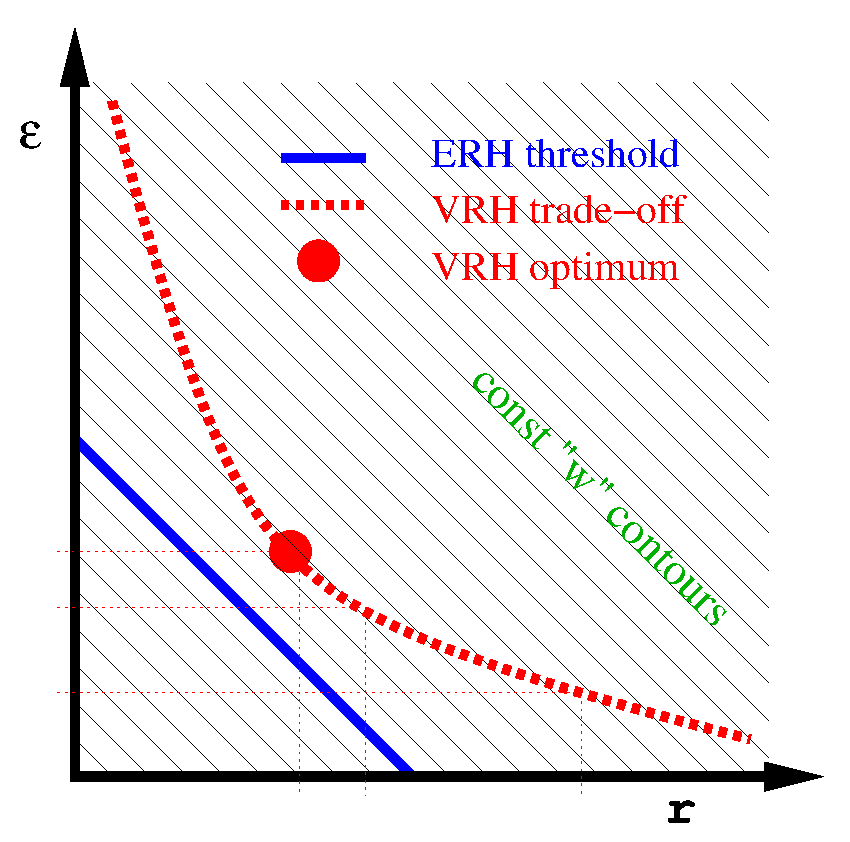
\includegraphics[width=0.4\hsize]{wdiagrm}

\caption{Comparing the VRH with the ERH procedure. 
The solid blue line that corresponds to the ERH threshold $w_c$ 
encloses an ``area" that corresponds to $n_c$. 
The VRH trade-off is represented by the dashed red line. 
The VRH optimum is represented by the thick red dot.
The VRH-to-ERH consistency requirement \Eq{e46} 
is to have the VRH optimum sitting on on the solid blue line.}
\label{fv}
\end{figure}


\hide{
%%%%%%%%%%%%%%%%%%%%%%%%%%%%%%%%%%%%%%
\begin{figure}[H]

\includegraphics[width=0.5\hsize]{ptsD_lattice}

\caption{The diffusion coefficient for the 2D lattice model. 
The dots are determined from the spectral analysis.
The lines are the ERH estimate. The thick line and its 
corresponding dots are for a network whose $\epsilon$ 
has uniform distribution within ${[0,\sigma]}$. 
The thin line and its corresponding dots are for 
a modified distribution that has same median. 
See text for details. The ERH estimate is sensitive 
enough to discriminate the two networks.
}
\label{f3}
\end{figure}
}


%%%%%%%%%%%%%%%%%%%%%%%%%%%%%%%%%%%
\begin{figure}[H]

\mpg[2cm]{(a) \\ \vspace*{2cm}} 
\includegraphics[width=0.7\hsize]{ptsD_Banded_Image}

\mpg[2cm]{(b) \\ \vspace*{4cm}} 
\includegraphics[width=0.7\hsize]{ptsD_Banded}

\mpg[2cm]{(c) \\ \vspace*{4cm}} 
\includegraphics[width=0.7\hsize]{ptsD_Banded_scatter}

\caption{
We consider a quasi 1D network that is described 
by sparse banded matrix. The bandwidth is~$b$, 
and the log-width of the rate distribution is~$\sigma$.  
See text for details.
%
{\bf \ (a)} The numerical result for $g_s=D/D_{\tbox{linear}}$ 
imaged as a function of $\sigma$ and $b$.
The values of $D$ are found via a numerical 
resistor network calculation.  
%
{\bf \ (b)} Plot of the subset of results that 
refer to the $b=10$ matrix. 
The curve is the ERH prediction. 
%
{\bf \ (c)} Scatter diagram that shows 
the correlation between the "$D$" that is extracted 
from the spectral analysis, and the $D$ that  
has been found via the resistor network calculation.}
\label{f4}
\end{figure}



%\end{widetext}

%%%%%%%%%%%%%%%%%%%%%%%%%%%%%%%%%%%%%%%%%%%%%
%%%%%%%%%%%%%%%%%%%%%%%%%%%%%%%%%%%%%%%%%%%%%
\end{document}


